\documentclass[letterpaper, 12pt]{article}
\usepackage{fullpage}
\usepackage{cite}
\usepackage{graphicx}
\graphicspath{ {images/} }

\begin{document}

\title{Graph Isomorphism}
\author{Franklin van Nes}
\date{Tuesday 12th November, 2017}
\maketitle

\begin{enumerate}
    \item Formally define and describe the topic (whether technique, algorithm, model or class) in detail, and discuss its significance.
    \\
    Graph Isomorphism is very much defined in its name: Iso (same) morphism (shape) of graphs.
    In more detail, two finite graphs are isomorphic if they share the same number of vertices connected in the same way.
    Formally, two finite graphs $G$ and $H$ with graph vertices $G.V$ and $H.V$ labelled $V_n = \{1, 2, 3, 4, ... , n\}$, and graph edges $G.E$ and $H.E$
    are said to be isomorphic if $f: G.V \rightarrow H.V$ is an edge-preserving bijection. Meaning
    that there exists a permutation $p$ of $V_n$ so that edges $(u, v) \in G.E \iff (p(u), p(v)) \in E.V$ ~\cite{gary-definer}.
    Figure \ref{graph-iso-image-figure} shows how two isomorphic graphs can look very different while still maintaining the same structure.

    \item How do you show a problem is in the class?
    While graph isomorphisms are quite clear in their classification as defined above, it should be noted that Graph Isomorphism
    falls into its own category of problem complexity, called \textit{Graph Isomorphism Complete}.
    According to Lubiw, it has yet to fall into a typical classification, and is neither P nor NP-complete ~\cite{anna-complexity}.
    There exists no known P algorithm, yet graph isomorphism has not be shown to be NP-complete. This means that either a P algorithm
    must exist for graph isomorphism, graph isomorhpism is a problem outside of P and NP, or, as Schöning argues, Graph isomorphism problems are in the low hierarchy of NP,
    which "does not equal NP unless the polynomial hierarchy collapses to the second level" ~\cite{np-hierarchy}.
    Deeper explanation of this exceeds the reaches of this paper, though Schöning's research is well explained with the proper background.
    \item Which are representative or classic problems in this class?
    \item How does this class compare to other classes?
    \item What techniques are used to solve problems in this class?

\end{enumerate}
\section{Figures}
\begin{figure}[p]
    \label{graph-iso-image-figure}
    \caption{Two isomorphic graphs. The colors indicate matching vertices, even
    if their labels do not match. ~\cite{wikimedia-images}}
    \centering
    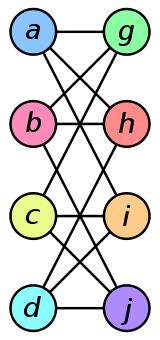
\includegraphics[scale=0.4]{graph-iso-a}
    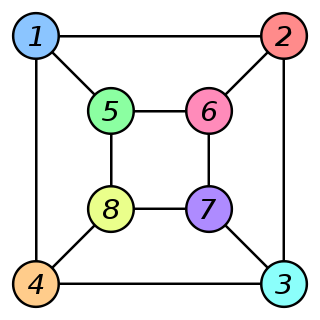
\includegraphics[scale=0.4]{graph-iso-b}
\end{figure}

\bibliography{mybib}{}
\bibliographystyle{abbrv}
\end{document}
